\documentclass[dvisvgm,multi=true]{standalone}
\usepackage{mathmlcoresvg}
\begin{document}
% <figcaption><span>Figure 15: </span>Box model for the <code>top</code>
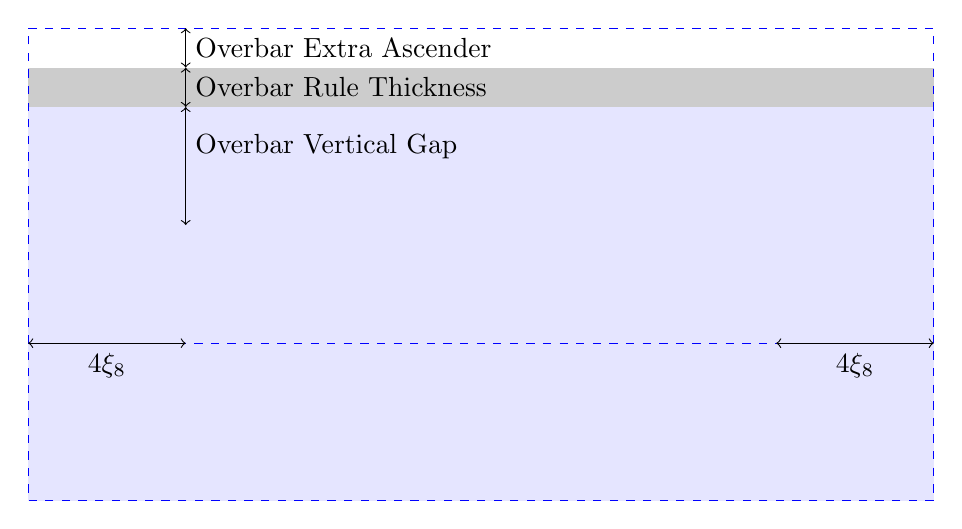
\begin{tikzpicture}[yscale=-1]

  \fill[blue!10] (0,-3.5) -- (11.5,-3.5) -- (11.5,2) -- (0,2) -- cycle;
  \MathMLBox{2}{0}{1.5}{1}{red}
  \fill[black!20] (0,-3.5) -- (11.5,-3.5) -- (11.5,-3) -- (0,-3) -- cycle;

  \draw[dashed,blue](0,-4) -- (11.5,-4) -- (11.5,2) -- (0,2) -- cycle
  (0,0) -- (11.5,0);

  \draw[<->] (2,-3) -- (2,-2.5) node[right]{Overbar Vertical Gap} -- (2,-1.5);
  \draw[<->] (2,-3) -- (2,-3.25)
    node[right]{Overbar Rule Thickness} -- (2,-3.5);
  \draw[<->] (2,-4) -- (2,-3.75)
    node[right]{Overbar Extra Ascender} -- (2,-3.5);

  \draw[<->] (0,0) -- (1,0)node[below]{$4\xi_8$} -- (2,0);
  \draw[<->] (9.5,0) -- (10.5,0)node[below]{$4\xi_8$} -- (11.5,0);
\end{tikzpicture}

\end{document}
